% Options for packages loaded elsewhere
\PassOptionsToPackage{unicode}{hyperref}
\PassOptionsToPackage{hyphens}{url}
%
\documentclass[
]{book}
\usepackage{lmodern}
\usepackage{amsmath}
\usepackage{ifxetex,ifluatex}
\ifnum 0\ifxetex 1\fi\ifluatex 1\fi=0 % if pdftex
  \usepackage[T1]{fontenc}
  \usepackage[utf8]{inputenc}
  \usepackage{textcomp} % provide euro and other symbols
  \usepackage{amssymb}
\else % if luatex or xetex
  \usepackage{unicode-math}
  \defaultfontfeatures{Scale=MatchLowercase}
  \defaultfontfeatures[\rmfamily]{Ligatures=TeX,Scale=1}
\fi
% Use upquote if available, for straight quotes in verbatim environments
\IfFileExists{upquote.sty}{\usepackage{upquote}}{}
\IfFileExists{microtype.sty}{% use microtype if available
  \usepackage[]{microtype}
  \UseMicrotypeSet[protrusion]{basicmath} % disable protrusion for tt fonts
}{}
\makeatletter
\@ifundefined{KOMAClassName}{% if non-KOMA class
  \IfFileExists{parskip.sty}{%
    \usepackage{parskip}
  }{% else
    \setlength{\parindent}{0pt}
    \setlength{\parskip}{6pt plus 2pt minus 1pt}}
}{% if KOMA class
  \KOMAoptions{parskip=half}}
\makeatother
\usepackage{xcolor}
\IfFileExists{xurl.sty}{\usepackage{xurl}}{} % add URL line breaks if available
\IfFileExists{bookmark.sty}{\usepackage{bookmark}}{\usepackage{hyperref}}
\hypersetup{
  pdftitle={Bahamas Guide for Applicants for Research and ABS Permits},
  hidelinks,
  pdfcreator={LaTeX via pandoc}}
\urlstyle{same} % disable monospaced font for URLs
\usepackage{longtable,booktabs}
\usepackage{calc} % for calculating minipage widths
% Correct order of tables after \paragraph or \subparagraph
\usepackage{etoolbox}
\makeatletter
\patchcmd\longtable{\par}{\if@noskipsec\mbox{}\fi\par}{}{}
\makeatother
% Allow footnotes in longtable head/foot
\IfFileExists{footnotehyper.sty}{\usepackage{footnotehyper}}{\usepackage{footnote}}
\makesavenoteenv{longtable}
\usepackage{graphicx}
\makeatletter
\def\maxwidth{\ifdim\Gin@nat@width>\linewidth\linewidth\else\Gin@nat@width\fi}
\def\maxheight{\ifdim\Gin@nat@height>\textheight\textheight\else\Gin@nat@height\fi}
\makeatother
% Scale images if necessary, so that they will not overflow the page
% margins by default, and it is still possible to overwrite the defaults
% using explicit options in \includegraphics[width, height, ...]{}
\setkeys{Gin}{width=\maxwidth,height=\maxheight,keepaspectratio}
% Set default figure placement to htbp
\makeatletter
\def\fps@figure{htbp}
\makeatother
\setlength{\emergencystretch}{3em} % prevent overfull lines
\providecommand{\tightlist}{%
  \setlength{\itemsep}{0pt}\setlength{\parskip}{0pt}}
\setcounter{secnumdepth}{5}
\usepackage{booktabs}
\ifluatex
  \usepackage{selnolig}  % disable illegal ligatures
\fi
\usepackage[]{natbib}
\bibliographystyle{apalike}

\title{Bahamas Guide for Applicants for Research and ABS Permits}
\author{}
\date{\vspace{-2.5em}16-02-2021}

\begin{document}
\maketitle

{
\setcounter{tocdepth}{1}
\tableofcontents
}
\hypertarget{welcome}{%
\chapter*{Welcome}\label{welcome}}
\addcontentsline{toc}{chapter}{Welcome}

Welcome to the Bahamas Research Permit and Access and Benefit Sharing (ABS) System guide for applicants.

This guide has been prepared as a practical guide to assist you through each step of the online research permit and ABS system. The guide will take you through:

\begin{itemize}
\tightlist
\item
  Documents you need to provide
\item
  Each step in the online system
\item
  Expectations about project impact and benefit-sharing under the Nagoya Protocol
\end{itemize}

This is a practical guide to applying for a research permit in the Bahamas through its online system. It is not a guide to the laws and regulations of the Bahamas. Applicants seeking clarification on legal issues are advised to contact the appropriate authorities in the Bahamas and to seek appropriate specialist legal advice.

\hypertarget{introduction}{%
\chapter*{Introduction}\label{introduction}}
\addcontentsline{toc}{chapter}{Introduction}

The Bahamas Research and Access and Benefit-Sharing Permit System provides a one stop shop to obtain all the main permits needed to conduct research involving biodiversity and genetic resources in the Bahamas. As you complete the application the system will automatically determine which standard permits you need and pre-fill them for you. We also provide information on specialist permits that you may require. Your profile and pre-filled permits will then be sent to desk officers at DEPP who will direct your application to the appropriate departments.

The system is designed to streamline the application process, making it easy to apply for all the major permits associated with typical research projects. At the same time, the system addresses access to genetic resources and benefit-sharing under the \href{https://www.cbd.int/abs/}{Nagoya Protocol} of the \href{https://www.cbd.int/}{United Nations Convention on Biological Diversity}. This involves a contractual agreement between your home institution and the government of the Bahamas in the interest of ensuring equitable outcomes for researchers and communities and biodiversity in the Bahamas.

\hypertarget{registering-your-user-profile-and-logging-in}{%
\chapter*{Registering Your User Profile and Logging in}\label{registering-your-user-profile-and-logging-in}}
\addcontentsline{toc}{chapter}{Registering Your User Profile and Logging in}

\hypertarget{orcid-id}{%
\subsection{ORCID ID}\label{orcid-id}}

Applicants will need to use a free ORCID ID to create a profile. ORCID stands for Open Researcher and Contributor ID. ORCID's mission is to enable transparent and trustworthy connections between researchers, their contributions, and their affiliations by providing a unique, persistent identifier for researchers to use free of charge - as they engage in research, scholarship, and innovation.

If you already have an ORCID ID please use that. Please do not create a second one.

If you do not have an ORCID ID you can set one up \href{https://orcid.org/}{here}. An ORCID profile is under the control of the researcher themselves and they retain the capacity to make information public or private.

ORCID ids distinguish researchers from others who might have the same or similar names. They also keep researchers connected to their work, regardless of name changes or changes to organizational affiliation. These ids link researchers and their scholarly activities - like published articles or dissertations, patents, artistic performances and datasets. The advantage of ORCID ids for researchers are that they allow information on their employment, research funding and publications to be stored in one place. In particular, the publication profile can be automatically updated through services such as Crossref. This makes it easier for us to create an electronic archive of research publications about the Bahamas and reduces the need to send emails asking for copies of publications.

When you have logged in for the first time using ORCID you will need to fill out a user profile.

\hypertarget{user-profile}{%
\section{User Profile}\label{user-profile}}

This section covers the steps necessary to register your user profile with the Bahamas Research and Access and Benefit-Sharing Permit System. When registering you will create a free username and password with your email address. You will register your profile using the registration page below:

\begin{figure}
\centering
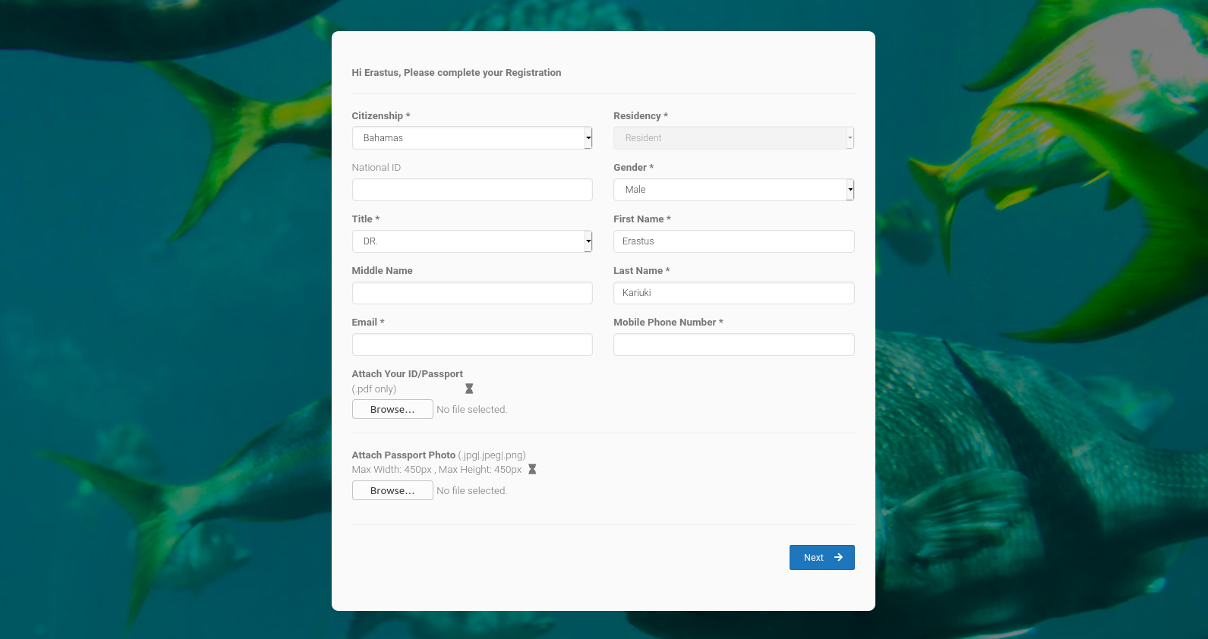
\includegraphics{images/account_registration.png}
\caption{Account registration page}
\end{figure}

To complete the registration you will need the following documents:

\hypertarget{a-photocopy-of-your-passport}{%
\subsection{A Photocopy of Your Passport}\label{a-photocopy-of-your-passport}}

This should be your current passport and it should be in pdf format. Your passport is required as part of the registration process and will be needed to create your account.

\hypertarget{passport-sized-photo}{%
\subsection{Passport Sized Photo}\label{passport-sized-photo}}

You are required to provide a passport photo as part of the registration process. The standard passport photo size for the Bahamas is the same as in the United States and European Union countries (sizes below). You will be able to upload, recentre and crop the photo using our photo crop functionality.

\begin{figure}
\centering
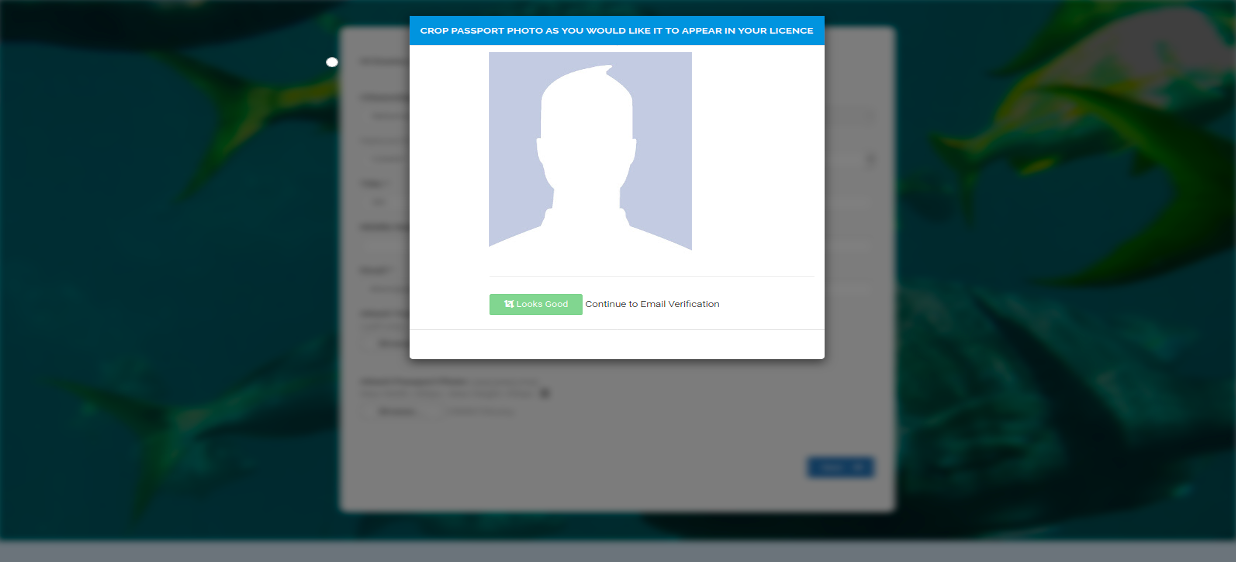
\includegraphics{images/passport_photo.png}
\caption{Passport photo upload}
\end{figure}

\textbf{Electronic image requirements}

\begin{itemize}
\tightlist
\item
  The format should be jpeg or png
\item
  Minimum size 600 pixels by 600 pixels, maximum size 1200 by 1200 pixels.
\item
  The image must be in colour (24 bits per pixel) in sRGB colour space.
\end{itemize}

\textbf{Scanning an existing image}

If you are scanning an existing image the photo itself must be:

\begin{itemize}
\tightlist
\item
  51mm x 51mm (2 x 2 inches)
\item
  Scanned at a resolution of 300 pixels per inches (or 12 pixels per millimetre)
\end{itemize}

Upon successful registration with the ABS permit system, a verification code window will open and you will have to enter a code sent to the email address you have provided. Once you have done this successfully, you will be taken to the ABS permit application form.

\hypertarget{logging-in}{%
\section{Logging in}\label{logging-in}}

Once you have registered your profile, you can log in through the Bahamas Access and Benefit Sharing System Home page. You can log in using your ORCID id.

\hypertarget{your-home-page}{%
\section{Your Home Page}\label{your-home-page}}

When you have logged into the system you will be taken to your home page. From here you will be able to create new applications, retrieve the details of existing applications and review invoices for application fees.

\hypertarget{communications-with-desk-officers}{%
\section{Communications with Desk Officers}\label{communications-with-desk-officers}}

The desk officers at permit granting authorities may need to contact you with questions relating to your application. This is handled through emails generated by the system. These communications are automatically stored as part of the file history of the application.

\hypertarget{general}{%
\chapter{General}\label{general}}

At the beginning of the application you will answer a set of trigger questions. This section helps the system to determine what permits you will need for your proposed project. It is composed of simple `yes/no' questions. An answer is required to each question in order to determine which permits you are likely to need and as a result, which parts of the form you should answer. If you answer `No' to the first three questions, you will be taken out of the system as your research does not relate to biological material or Access and Benefit Sharing in the Bahamas. If this is the case, you must apply directly through the appropriate government departments. In a small number of cases you may need a specialised permit that is not included in the online system. You can find these and links to the forms in the \href{https://www.bahamas.gov.bs/wps/portal/public/Permits\%20and\%20Licences/!ut/p/b1/vVTJcptAEP0Wf0DMDDAsR_adQSyS4KICYRCbBEIbfH1wkoOdqtiX2DOnqXndr_v1QiTElkiO6a0q00t1Oqbt6zthdhTQHEGgOUdDgAFG5NmCx-okhmgBxB8AaPDbXsO0oyzfWJUEYECF1qmVTIEAEBtiG8YTL43GXVWSoo9u2l5z0lCE6mBcqxJc2UBHV7KskB1R9x8rMj_aaMaeLEoWrsc-TsQqu9Y7xG_SslSDpKJi8g66m4bOPTcwG37nOeHl4dtZOSN0iPNm9BzRDTMYzSdn_2LmR8-_M2I2ZPOoy_tBtBgJXh6xp6tnVtVT_iQZQmtTuOCEK5VtXeHp6U_e4B9HAJ_pZhJJlXXP9333DJ4hBVlIQpZmWZZHCDKLLMmHHizyE8Cr8r8AH4QYLwD2jYdwDZbiAMEP4ApwLiRCYgvoXVBPvTE3s1_PK8qtTdPJTAM2AATRLXSjZnb53A2VAUIFWqFszEFtkKECXTeXvXztR6IgT7BS478JMRnyC6EEGStCSzPQX02oIcwtGrGhJyASaBh-NyH1rZJqHgZfnuG7pqFX_7-G7yaF4xmIWI7mOQbQNMcS6zpmeHnZHorhFv3-6vKyNRuBH1edWFoqXHUHZPXevcfJeeIbv403Ysl1OTvaut6RKd48hDKouou2Js9liR8Yj3Nl1pKoWYHtNWspXlnHsZnlahxrmTTArr1TFD8pVjJwbdgPQ4MO54a5zFlRWHoj41z7MRz7WrJug8EeCpKz6rAdgtsay0bXnovT_rxWffPaTHKrTdSh3kluvdMag12iorKhndJy2TCufupeiL6LbjYylcJ9e-mnn3zSVbg!/dl4/d5/L2dBISEvZ0FBIS9nQSEh/\#}{Permits and Licences} section of the Government website.

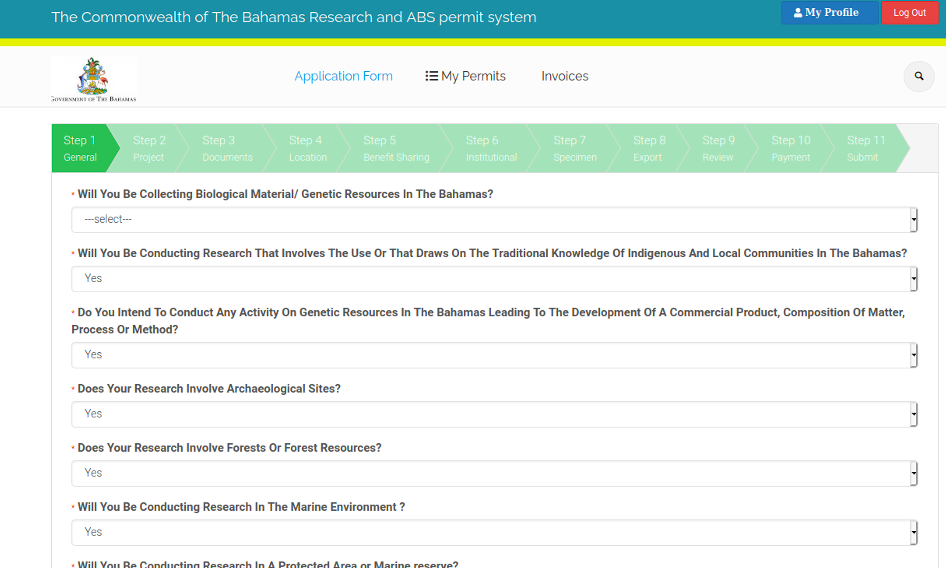
\includegraphics{images/trigger_questions.png}
The following is a breakdown of each trigger question at the start of the application form, including the rationale. The first three questions determine whether the Bahamas Access and Benefit Sharing System is the appropriate portal for an applicant to use to gain research permits for their specific research project.

\hypertarget{will-you-be-collecting-biological-materialgenetic-resources-in-the-bahamas}{%
\section{Will You Be Collecting Biological Material/Genetic Resources In The Bahamas?}\label{will-you-be-collecting-biological-materialgenetic-resources-in-the-bahamas}}

If you are \emph{not} collecting biological material in the Bahamas, you do not need to obtain permits through the Bahamas ABS system and should obtain your permits directly. Biological material refers to any specimen taken from a biological organism of any kingdom, including animals, plants, fungi, bacteria, chromists and archaea. Genetic resources refers to biological material of actual or potential value. To collect these materials means to remove them from their place of origin, it does not refer to the study of biological material previously obtained by other parties. There is a distinction between the collection and the export of biological materials (See question 1.9)

\hypertarget{will-you-be-conducting-research-that-involves-the-use-of-or-draws-on-the-traditional-knowledge-of-indigenous-peoples-and-local-communities-in-the-bahamas}{%
\section{Will You Be Conducting Research That Involves The Use of Or Draws On The Traditional Knowledge Of Indigenous Peoples And Local Communities In The Bahamas?}\label{will-you-be-conducting-research-that-involves-the-use-of-or-draws-on-the-traditional-knowledge-of-indigenous-peoples-and-local-communities-in-the-bahamas}}

In its working practice the Convention on Biological Diversity and its Nagoya Protocol use the term indigenous peoples and local communities. If you will be conducting research that involves communities in the Bahamas you need to answer yes to the above question.

Bahamian communities have a rich and diverse cultural heritage that deserves to be recognised, valued, protected and promoted. Traditional knowledge refers to knowledge, innovations and practices that are passed down and adapted and developed across generations to form part of the living traditions and heritage of the communities of the Bahamas.

If you intend to conduct research that involves interviews, recordings, photography, film or engagement activities involving communities, families or individuals you should answer yes to the above question. You will be expected to conduct your research in a way that fully respects the human rights of community members and in accordance with professional ethical standards. If you are unsure about this you should seek guidance.

If your research will involve filming activity you will need to apply for a permit from the Bahamas Film and Television Commission in addition to the permits required for your research. You can apply for that permit \href{http://www.bahamasfilm.com/Resources/procedures.htm}{here}.

\hypertarget{do-you-intend-to-conduct-any-activity-on-genetic-resources-in-the-bahamas-leading-to-the-development-of-a-commercial-product-composition-of-matter-process-or-method}{%
\section{Do You Intend To Conduct Any Activity On Genetic Resources In The Bahamas Leading To The Development Of A Commercial Product, Composition Of Matter, Process Or Method?}\label{do-you-intend-to-conduct-any-activity-on-genetic-resources-in-the-bahamas-leading-to-the-development-of-a-commercial-product-composition-of-matter-process-or-method}}

This question relates to your intentions with any biological material or information you may collect in the Bahamas. Commercial products are products which are sold to the general public, or to industry. Compositions of matter, processes and methods are categories of things which can be patented. Compositions of matter relate to tangible compositions - where the patent is for a material thing. Compositions of process or method relate to a way to use a product or serious of steps to accomplish a result. You should answer yes to this question if you have any intention of using research on genetic resources in the Bahamas to develop and/or patent a product of any kind for commercial sale. If you wish to profit commercially from biological material or information obtained in the Bahamas, a contract (often called Mutually Agreed Terms or an ABS agreement) will need to be established with the Government of the Bahamas before research begins.

\hypertarget{does-your-research-involve-archaeological-sites}{%
\section{Does Your Research Involve Archaeological Sites?}\label{does-your-research-involve-archaeological-sites}}

An archaeological site is any place where there are physical remains of past human activities. If you are doing research in an archaeological site, you will need a permit from the Antiquities Monuments \& Museums Corporation. This permit is part of the system and will be autofilled as you complete this form. AMMC desk officers will contact you if they need further clarification on your proposed research.

\hypertarget{does-your-research-involve-forests-or-forest-resources}{%
\section{Does Your Research Involve Forests Or Forest Resources?}\label{does-your-research-involve-forests-or-forest-resources}}

The Department of Forestry does not currently issue permits but will do so in the future. As a result, this question is for informational purposes only.

\hypertarget{will-you-be-conducting-research-in-the-marine-environment}{%
\section{Will You Be Conducting Research In The Marine Environment?}\label{will-you-be-conducting-research-in-the-marine-environment}}

Any research conducted in Marine Environments within and around the Bahamas must be sanctioned by the Department of Marine Resources. These permits form part of this system and will be autocompleted as you proceed through the system.

\hypertarget{will-you-be-conducting-research-in-a-protected-area-or-marine-reserve}{%
\section{Will You Be Conducting Research In A Protected Area or Marine reserve?}\label{will-you-be-conducting-research-in-a-protected-area-or-marine-reserve}}

In the Bahamas there are marine protected areas and forested protected areas. Permits will be needed to conduct research in any protected area managed by Bahamian public authorities. If your research will be conducted in any protected area or marine reserve managed by the state of the Bahamas you must select yes here.

\hypertarget{will-your-research-involve-the-use-of-cites-listed-resources}{%
\section{Will Your Research Involve The Use Of CITES Listed Resources?}\label{will-your-research-involve-the-use-of-cites-listed-resources}}

CITES stands for the Convention on International Trade in Endangered Species. It is a multilateral treaty to protect endangered plants and animals. Trade in species listed in CITES Appendix I, II or III are heavily regulated. More information can be found on the \href{https://cites.org/}{CITES website}. You must click yes if you seek to collect biological material from CITES listed species. You will not be able to collect specimens related to these species without a CITES permit.

\hypertarget{will-you-be-exporting-biological-materialgenetic-resources-from-the-bahamas}{%
\section{Will You Be Exporting Biological Material/Genetic Resources From The Bahamas?}\label{will-you-be-exporting-biological-materialgenetic-resources-from-the-bahamas}}

Specify whether your research will involve the removal of biological samples from the Bahamas. This refers not only to physical samples, but also to genetic sequence data (also known as digital sequence information) that you may seek to extract and upload to a database or otherwise transport outside the jurisdiction of the Government of the Bahamas. The export of any genetic material from the Bahamas must be accompanied by an appropriate permit.

\hypertarget{project-information}{%
\chapter{Project Information}\label{project-information}}

In this step you will provide information about your project including your research goals, sources of funding and the members of your research team.

\hypertarget{you-are-applying-as}{%
\section{You Are Applying As}\label{you-are-applying-as}}

In this section, you define what type of applicant you are. In answering this question you have the option to apply as:

\begin{itemize}
\tightlist
\item
  A Company
\item
  A Consortium (a consortium is a group of public or private entities)
\item
  An Individual
\item
  A Research Institution
\item
  A Student
\end{itemize}

The application form is the same regardless of the category of applicant. Please choose the category that most accurately reflects your status.

\begin{itemize}
\tightlist
\item
  If you are part of a consortium we will ask for details of the entities involved in the consortium. This includes all public and private entities.
\item
  If you are a company planning to conduct commercial research on biodiversity and/or traditional knowledge the application requirements are the same but the contractual provisions in the access and benefit-sharing agreement will normally be tailored to your project.
\end{itemize}

\hypertarget{institution-details}{%
\section{Institution Details}\label{institution-details}}

\textbf{Name of the Institution} - The name formally used for your institution.

\textbf{Institution Contact Person} - This is the legal officer (such as the contracts officer) who has authority to sign legally binding contracts on behalf of the institution. Unless you are that person you should not place your name here. Researchers are agents of their employers and do not normally possess legal authority to sign contracts on behalf of their institution.

\textbf{Institution Legal Registration Number} - This is the number or identifier used on the registration certificate for your organisation (e.g.~as used by Companies House or equivalent).

\hypertarget{research-team-details}{%
\section{Research Team Details}\label{research-team-details}}

\begin{figure}
\centering
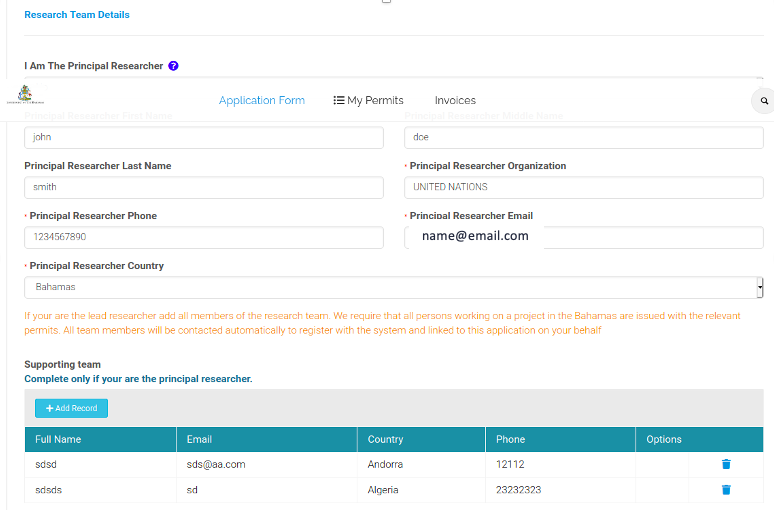
\includegraphics{images/research_team_details.png}
\caption{Research Team Details}
\end{figure}

If you are the principal researcher or team leader you need to provide the name and contact details of each member of your research team. The individuals will then be invited to register on the system and answer the relevant questions. The individuals will then be associated with the issued permits. All team members must be named on the permit at the point when it is issued. This cannot be rectified later.

Where an individual team member is from a different institution, their legal officer will also be required to sign an contract (ABS agreement).

Note that \textbf{all members of the research team must be named individuals} or processing of the application will be delayed for clarification.

\hypertarget{research-project-details}{%
\section{Research Project Details}\label{research-project-details}}

\begin{figure}
\centering
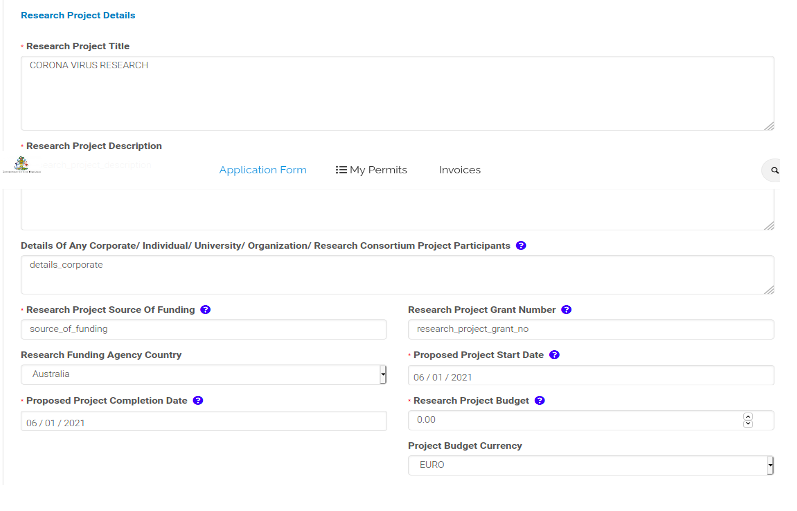
\includegraphics{images/research_project_details.png}
\caption{Research Project Details}
\end{figure}

\textbf{Research Project Description} This is a short abstract describing the project. It should be written in a form that is suitable for the general public to read.

\textbf{-Research Project Source of Funding} Please give the full name of the research funding organisation or other source of funding.

\textbf{Proposed Project Start Date}. This is the formal start date of the research project. It is not the start date of your proposed research in the Bahamas.

\textbf{Proposed Project Completion Date} This is the formal end date of the research project. It is not your proposed date of departure from the Bahamas.

\textbf{Research Project Grant Number}. This is the unique identifier awarded to your research grant when awarded by the funding agency. If you are presently at the application stage please use the application number.

If you have previously received a permit for research in the Bahamas please provide the number of the most recent permit that you received.

\hypertarget{equipment}{%
\section{Equipment}\label{equipment}}

These questions only apply in circumstances where you are seeking to make \emph{duty-free imports of equipment}. The term equipment does not apply to expendable supplies (food, fuels or other consumable materials etc.)

\hypertarget{documents}{%
\chapter{Documents}\label{documents}}

During this stage you will need the following documents:

\begin{itemize}
\tightlist
\item
  \textbf{Identification Document or Passport}
\item
  \textbf{Your CV}
\item
  \textbf{Your Institution Legal Registration Document}
\item
  \textbf{Research Proposal}
\item
  \textbf{Data Management Plan}
\item
  \textbf{Questionnaire Sample (where applicable)}
\end{itemize}

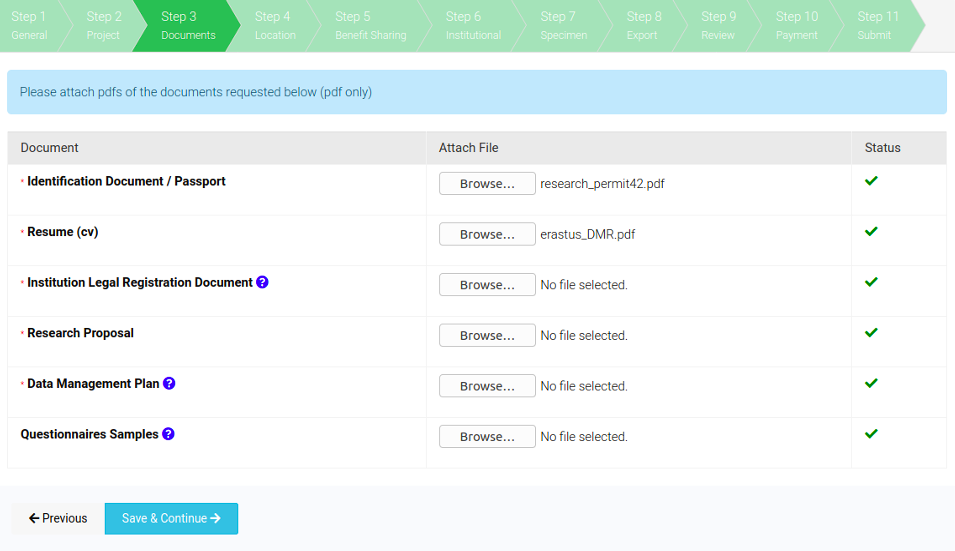
\includegraphics{images/documents.png}
\#\# Resume

\begin{itemize}
\tightlist
\item
  \textbf{Resume (Curriculum Vitae)} Your current CV. If you are leading a research team, provide only your own CV. You must also ensure you have included the contact details of your research team in step 2 - General Information. Research team members will each be invited to register with the system and to provide copies of their CVs by email.
\end{itemize}

\hypertarget{research-proposal-with-budget}{%
\section{Research Proposal with Budget}\label{research-proposal-with-budget}}

\begin{itemize}
\tightlist
\item
  \textbf{A copy of your research proposal and budget} This must include the budget as submitted or approved by the funding agency. It should also include details of any partner organisations (e.g.~all members of a consortium involved in the research).
\end{itemize}

\hypertarget{data-management-plan}{%
\section{Data Management Plan}\label{data-management-plan}}

\begin{itemize}
\tightlist
\item
  \textbf{Your Data Management Plan}. Before conducting your research you must plan how you will collect and store your data safely. This should include information on arrangements for the storage of specimens or samples that you propose to collect in the Bahamas and related data. This includes genetic sequence data (also known as digital sequence information). This also refers to matters of confidentiality for research projects involving interviews.
\end{itemize}

If you are unfamiliar with Data Management Planning the template for EU Horizon 2020 projects provides a useful guide and can be downloaded as a word document \href{https://ec.europa.eu/research/participants/data/ref/h2020/gm/reporting/h2020-tpl-oa-data-mgt-plan_en.docx}{here}. For US based researchers the National Science Foundation provides guidance on Data Management Planning in different subject areas. See the latest Directorate Wide Guidance for your subject area on the NSF website at \url{https://www.nsf.gov/bfa/dias/policy/dmp.jsp}.

All applicants are required to provide a data management plan.

\hypertarget{questionnaire-samples}{%
\section{Questionnaire Samples}\label{questionnaire-samples}}

If you will be conducting surveys or interviews as part of your research (e.g.~with community members, fishermen etc.) please provide samples of the proposed questionnaires.

\hypertarget{location}{%
\chapter{Location}\label{location}}

In this section you must provide location information for each site where research will be undertaken. The map provided allows you to select one or more research locations. Click save for each individual location in which you intend to conduct research before adding a new location.

To add locations, first click the `Add Location' button in blue. A window will pop-up, allowing you to insert the location details for your research in the three following ways:

\begin{itemize}
\tightlist
\item
  Dropping a Pin
\item
  Drawing a Polygon
\item
  Selecting National Parks
\end{itemize}

Please note that the location selector is powered by Google Maps. On odd occassions this may become unresponsive. Please be patient and retry where necessary. If you encounter persistent problems please raise an issue.

\begin{figure}
\centering
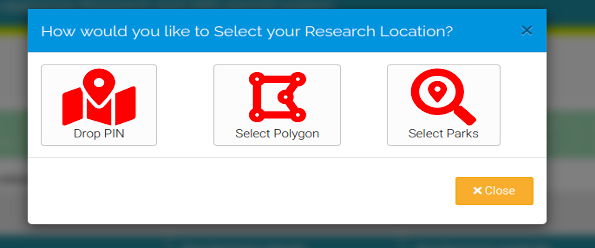
\includegraphics{images/Screenshot 2021-03-01 at 13.43.17.png}
\caption{Selecting a location}
\end{figure}

\textbf{Dropping a pin:} Through this method you can search the name of the location in which you wish to conduct research, suggestions will appear below the search bar, click on one of these suggestions and a pin will be dropped in that location on the map and the GPS co-ordinates will be entered into the form.

\textbf{Selecting a Polygon:} When you select this option, you will see three small icons at the top of the map, the hand, the polygon and the rectangle. Use the hand icon to drag the map, you can also zoom as necessary. Click the polygon icon to draw a polygon. When you are ready to draw a polygon, click once on the map, and release the mouse (do not attempt to drag) and your first polygon point will appear. Continue this step as many times as necessary, adding lines to the polygon. Ensure you click save otherwise your polygon co-ordinates will not be recorded. The system can only save one polygon at a time so ensure you click save. For good measure it is best to ensure you exit the pop-up and check that the record has been saved before proceeding with your next polygon.

\textbf{Selecting Parks:} If you select this option, all national parks will be highlighted when you open the map. Select the park(s) in which you wish to do research.

In this section, you must also provide information about where samples of biological material will be stored within the Bahamas. You must also provide the location of any field-stations which might be needed, and the number of full-time and part time staff expected to staff these locations.

\hypertarget{benefit-sharing}{%
\chapter{Benefit-Sharing}\label{benefit-sharing}}

The United Nations Convention on Biological Diversity (CBD) introduced the concept of benefit-sharing arising from the utilisation of genetic resources. In 2010 governments who are parties to the CBD adopted \emph{The Nagoya Protocol on Access to Genetic Resources and the Fair and Equitable Sharing of Benefits Arising from their Utilization.} Under the Nagoya Protocol governments may agree to grant prior informed consent to access genetic resources within their jurisdictions and to establish what are known as ``mutually agreed terms'' in the form of a contract on benefit-sharing with those seeking to use these resources for commercial or non-commercial purposes. An Annex to the Nagoya Protocol provides an indicative list of \href{https://www.cbd.int/abs/text/articles/?sec=abs-37}{Monetary and Non-monetary Benefits} that is useful in considering forms of benefit-sharing.

In practice, this means that \emph{all applicants} seeking to conduct research involving biodiversity or the traditional knowledge of communities in the Bahamas are required to set out the benefits that will be shared. Benefit-sharing as a concept can be considered similar to \emph{research impact} or \emph{project legacy} in that research is expected to have positive impacts for biodiversity and the communities of the Bahamas. This section of the application form asks you to quantify those benefits.

The estimated figure for benefit sharing is not an estimate of the general value accruing from the project (monetary or otherwise) rather it is an estimate of how much money will be spent in the Bahamas in the course of the project through defined activities and where relevant what will be shared with the Bahamas after the project. We are mindful that predicted costs of benefit sharing may change due to circumstances, however it is expected that applicants will make reasonable estimates and attempt to follow them through to the best of their ability. Please bear in mind that the data on benefit-sharing will form part of the contract negotiated with your institution. As such please make realistic assessments.

Benefit-sharing can take many forms and is commonly divided into \emph{monetary} and \emph{non-monetary} forms. Researchers seeking to conduct research in the Bahamas may also be at different stages in their careers with different means and budgets. Our expectations about benefit-sharing will recognise the diversity of means and will be proportionate to the means available to the individual and to the project. Our aim is to ensure a measurable return to the conservation of biodiversity in the Bahamas and for the benefit of Bahamian communities.

Expectations of researcher contribution will be assessed in accordance with their career status:

\begin{enumerate}
\def\labelenumi{\arabic{enumi}.}
\tightlist
\item
  \textbf{Early stage researchers} (such as undergraduates, masters students and PhD candidates) will be expected to think about how to offer benefits in kind. These might include contributions to community activities during the course of a research project or organising local events (such as a Cafe Scientifique) that contribute to community knowledge and understanding of biodiversity related research or benefit communities in the Bahamas in other ways.
\end{enumerate}

Researchers in this group are invited to list proposed activities and to provide estimates of the monetary value or its equivalent.

\begin{enumerate}
\def\labelenumi{\arabic{enumi}.}
\setcounter{enumi}{1}
\tightlist
\item
  \textbf{Established researchers} will generally hold significant research grants and may manage research teams. Researchers in this group may also lead or form part of consortiums of organisations including private sector entities.
\end{enumerate}

Researchers in this grouping will be expected to provide clear, quantifiable evidence of direct benefit-sharing in the Bahamas that will leave a measurable legacy. This should be reflected in budget allocations and the ability to calculate the percentage of the overall budget that will be spent on benefit sharing in the Bahamas.

Research activities involving benefit-sharing may include, but are not limited to:

\begin{itemize}
\tightlist
\item
  Workshops
\item
  Training courses
\item
  Conferences
\item
  Exchange Visits
\item
  Undergraduate, Masters, and PhD studentships
\item
  Equipment that remains in the Bahamas
\item
  Shared authorship of data and data products arising from research
\item
  Joint publications with local researchers (including publication costs for open access publications)
\item
  Joint ownership or control of intellectual property (know how, trade secrets, patents, copyright, trademarks, \emph{sui generis} database rights) arising from the utilisation of genetic resources
\end{itemize}

The distinction between purely non-commercial and commercial research has become increasingly blurred as a result of a drive to promote income generation from research activity (e.g.~arising from the Bayh-Dole Act). Applications that involve a commercial dimension will be expected to be explicit about proposed benefit-sharing with DEPP and the Government of the Bahamas.

Researchers whose work is explicitly commercial, involves a commercial dimension or commercial entities are encouraged to engage in consultations with DEPP at an early stage to facilitate agreement on an ABS contract.\\
3. \textbf{Commercial Activities}

Companies seeking to conduct research on biodiversity and genetic resources in the Bahamas are encouraged to contact DEPP at an early stage to discuss the terms of a possible contractual agreement. In addition to the options mentioned above, the following indicative list, provided with the Nagoya Protocol, may assist companies when entering into discussions with DEPP:

\begin{itemize}
\tightlist
\item
  Access fees/fee per sample collected or otherwise acquired;
\item
  Up-front payments;
\item
  Milestone payments;
\item
  Payment of royalties;
\item
  Licence fees in case of commercialization;
\item
  Special fees to be paid to trust funds supporting conservation and sustainable use of biodiversity;
\item
  Salaries and preferential terms where mutually agreed;
\item
  Research funding;
\item
  Joint ventures;
\item
  Joint ownership (or control) of relevant intellectual property rights.
\end{itemize}

Companies should note that while there will be an expectation of monetary benefit-sharing, non-monetary forms of benefit-sharing may also feature in an agreement.

\hypertarget{institutional-permits}{%
\chapter{Institutional Permits}\label{institutional-permits}}

In some cases institutions require answers to very specific questions. This section only lists questions that are not addressed elsewhere in the form and may appear disjointed for that reason.

If this section is blank simply press Save and Continue

The question required for a specific institutional permit is clearly indicated by a heading in red. The institutions in this step are: Bahamas National Trust (BNT), Department of Environmental Planning and Protection (DEPP), Department of Marine Resources (DMR), Department of Agriculture (DoA) and Antiquities, Monuments and Museums Corporation (AMMC).

\hypertarget{specimens}{%
\chapter{Specimens}\label{specimens}}

In this section, the applicant provides detail of species will be collected during their research project and go into more detail about what specifically they intend to collect. They will also specify whether they will be tagging specimens, and if so, the method of tagging.

\begin{figure}
\centering
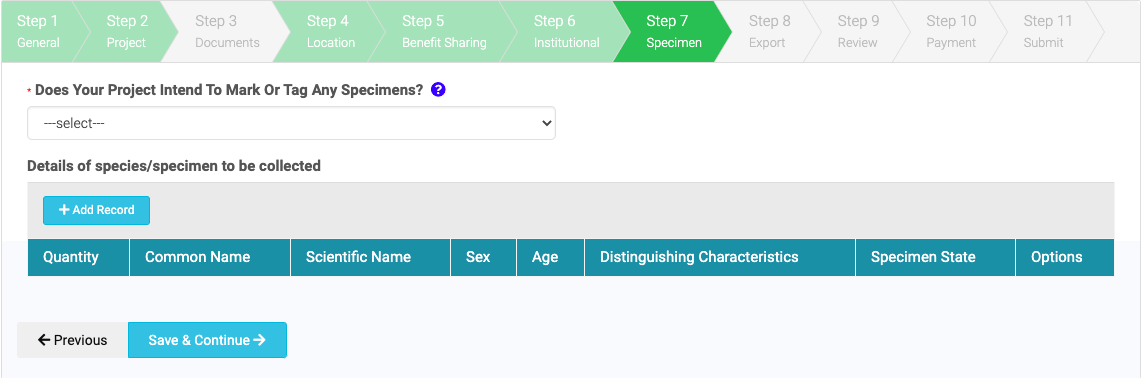
\includegraphics{images/specimen_section.png}
\caption{Step 7: Specimen}
\end{figure}

The page appears like so. To add details of a species or specimen to be collected click `Add Record' in blue. A new window will appear, through which you can add detailed information about specimens to be collected. Through this window you can specify the specimen quantity, common and scientific name, sex, age, distinguishing characteristics and specimen state. Specimen information must be added one record at a time. A summary of the record will appear in the portal once the record has been successfully saved.

For the question on the sex of a specimen please use NA if the organism does not have a sex (e.g.~in the case of fungi or bacteria) or if specimens are hermaphrodites.

\begin{figure}
\centering
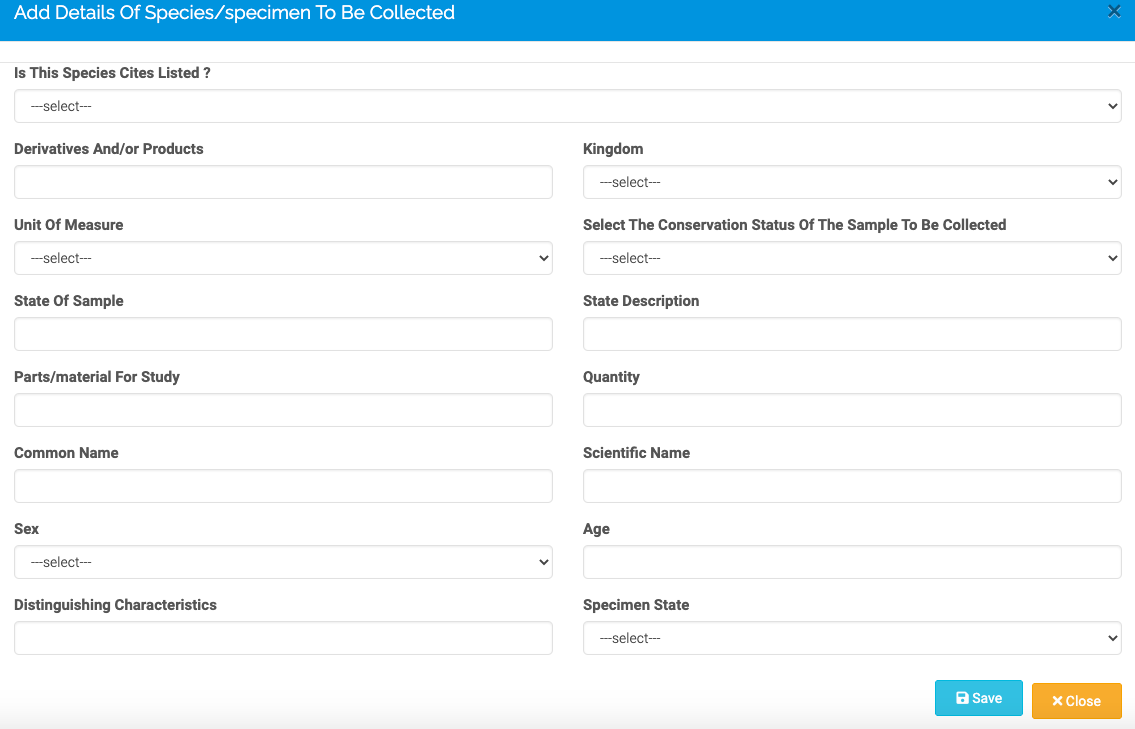
\includegraphics{images/species_form.png}
\caption{Species Form}
\end{figure}

\hypertarget{export}{%
\chapter{Export}\label{export}}

This step is only necessary for applicants who will be exporting biological/genetic material from the Bahamas. It is triggered when applicants answer `Yes' to the question `Will you be exporting Biological Material/Genetic Resources From The Bahamas?' in Step 1. If applicants select `No', this step in the application form will be inactive. When the applicants select `Yes' to the initial question, the following question will be asked: `Where applicable select the relevant marine organism export permit'. This question relates to the species for which specialist permits are required, these are:

\begin{itemize}
\tightlist
\item
  Permit to export marine mammals
\item
  Shark Export Permit
\item
  Turtle Export Permit
\end{itemize}

The questions that appear in this section will relate to whichever permit was selected. Please note, that to export CITES listed species, a CITES permit is required. Upon export of any other species from the Bahamas, an export permit will need to be obtained before departure.

\hypertarget{review}{%
\chapter{Review}\label{review}}

In the review stage you can review your answers for Steps 1-8 and a draft ABS Contract (also known as Mutually Agreed Terms). You can also download your pre-filled submission in the form of a pdf.

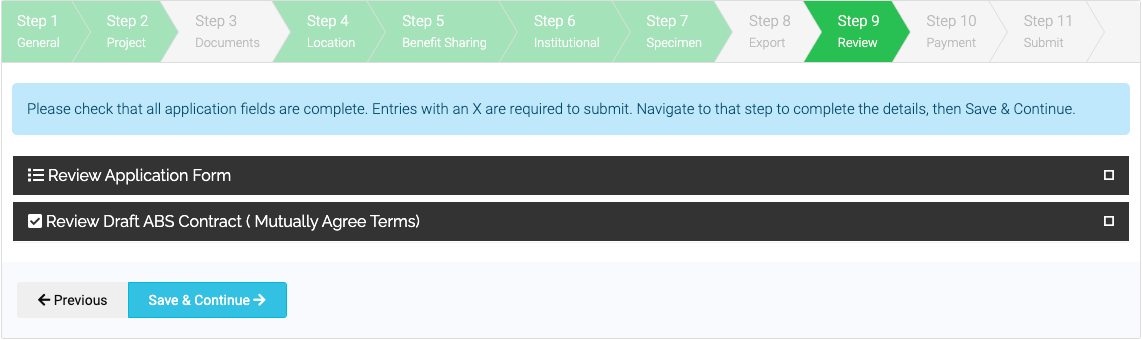
\includegraphics{images/review.png}
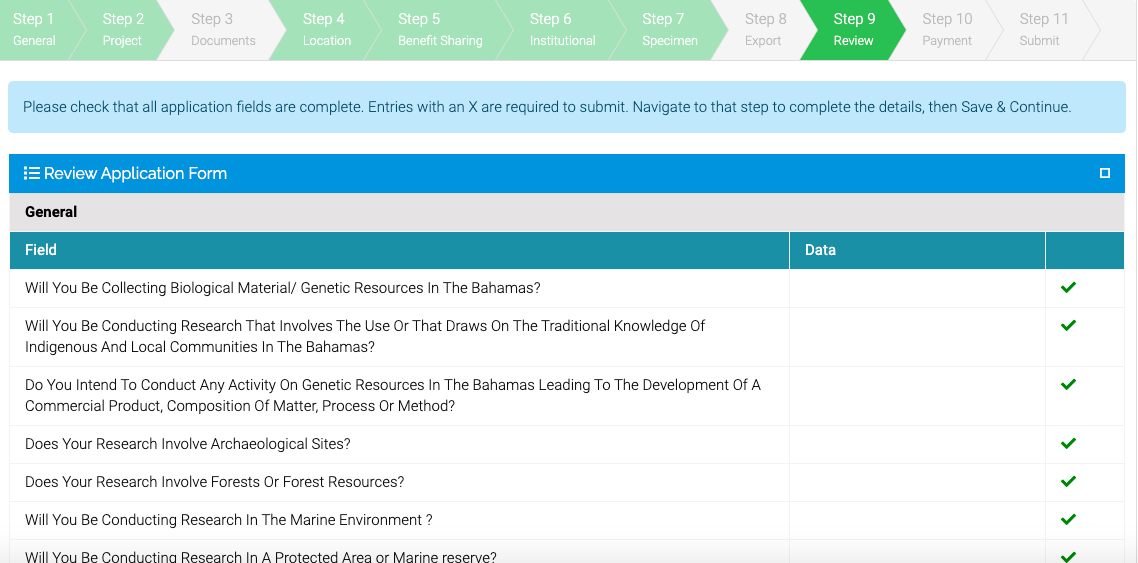
\includegraphics{images/review_application_form.png}

\begin{figure}
\centering
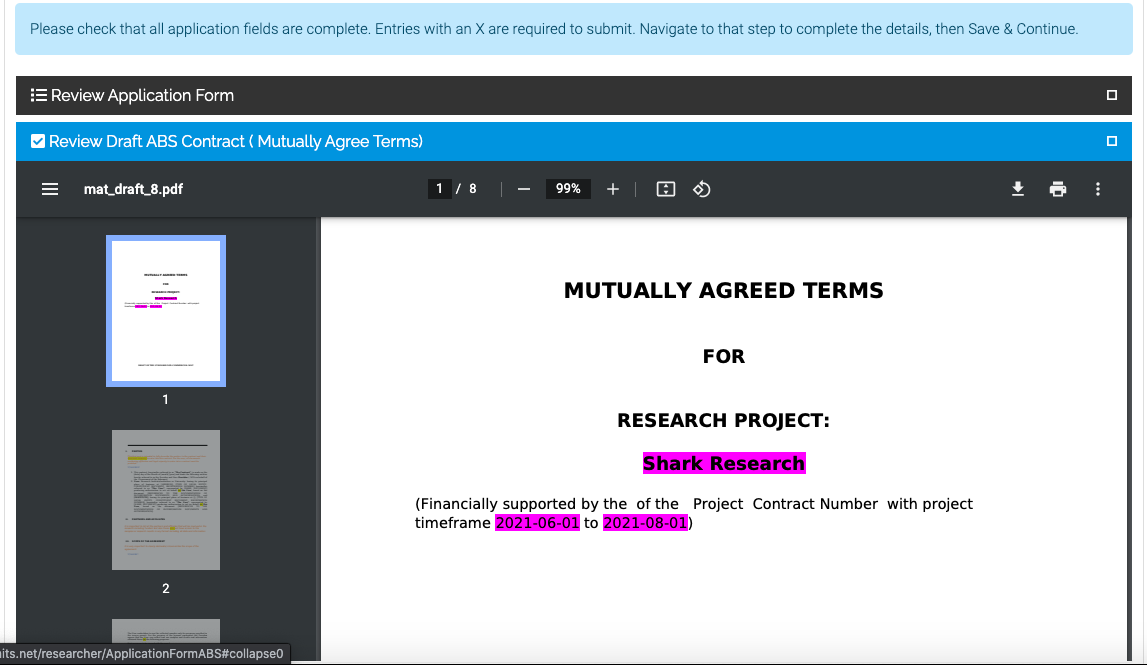
\includegraphics{images/review_mat.png}
\caption{In this stage you will also be able to see a draft ABS contract (Mutually Assured Terms) contract. This will be sent to the legal officer listed in the application at the time of submission as the basis for a contract. Please read the document to understand the nature of the obligations that you and your institution will be entering into}
\end{figure}

\hypertarget{payment}{%
\chapter{Payment}\label{payment}}

There is an annual fee of \$1,500 US per institution to use the The Bahamas Research and Access and Benefit-Sharing Permit System. This is a registration fee and not an application fee. Almost every permit the applicant requires will also have an attendant permit fee. You will receive emails notifying you of any application fees which need to be paid. You can also view all invoices in the `Invoices' section of your home page.

You can pay the registration fee through the system. By clicking `Accept and Invoice' you will be shown the amount to be invoiced. Clicking `Pay Now' you can pay via Bank Transfer, Credit Card, Paypal. If you have already paid, there is a facility to attach a pdf of evidence of payment (such as a bank deposit slip or credit card payment information)

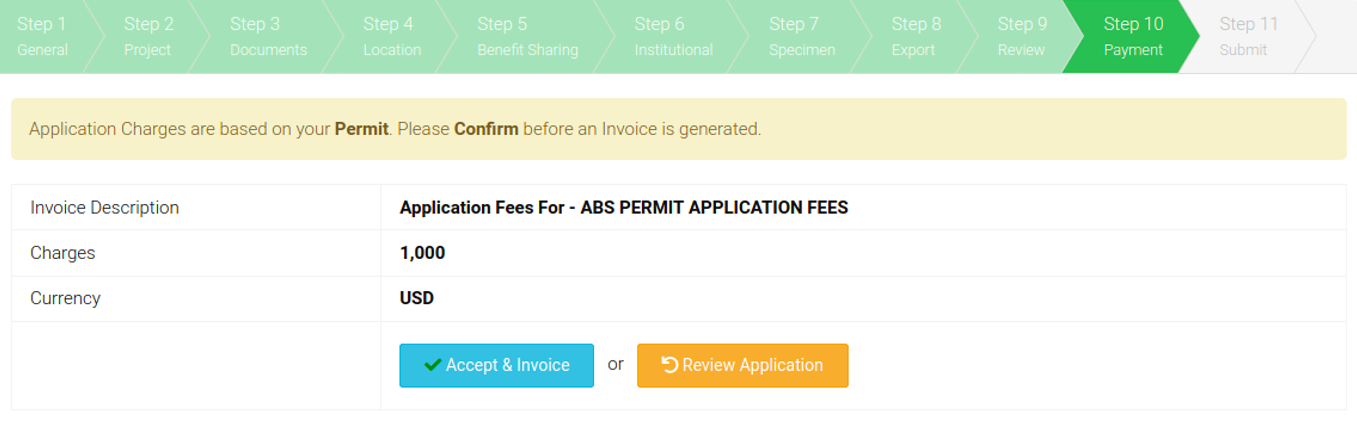
\includegraphics{images/payment1.png}
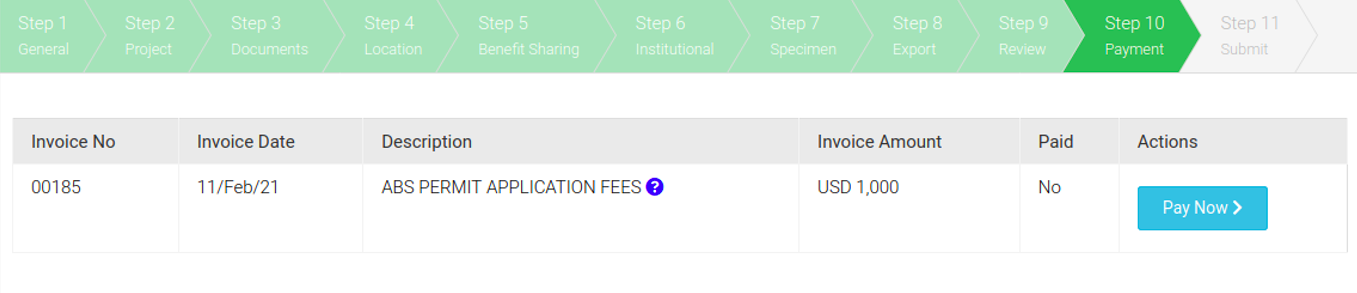
\includegraphics{images/payment2.png}
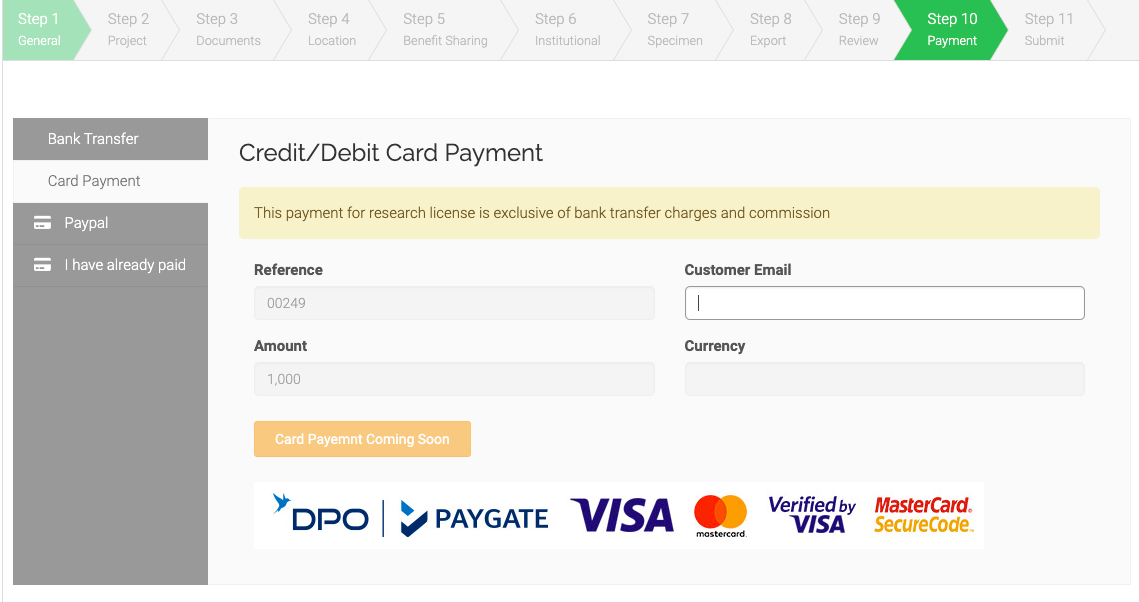
\includegraphics{images/payment3.png}

\hypertarget{step-11-submit}{%
\chapter{Step 11: Submit}\label{step-11-submit}}

In this stage you submit your application. Before submission applicants must agree to what is essentially the Terms and Conditions of the application process in the Bahamas. Applicants must:

\begin{itemize}
\tightlist
\item
  Certify that the information in their application is true accurate to the best of their knowledge
\item
  Agree to abide by the laws and regulations of the Bahamas
\item
  Agree to observe standards of best practice in animal welfare
\item
  Agree to observe standards of best practice in ethical conduct in research involving humans
\end{itemize}

The application cannot be submitted unless all four boxes have been checked.

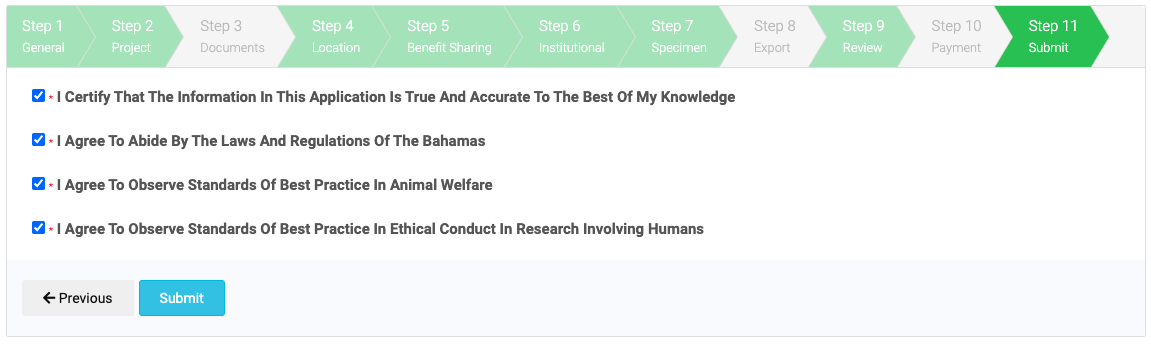
\includegraphics{images/submit.png}
When you are satisfied with your submission answers you are ready to submit your application. It is best to carefully examine application answers before submitting as it may not be possible to rectify mistakes later.

\hypertarget{what-happens-next}{%
\section{What Happens Next}\label{what-happens-next}}

Following the submission of your application you and your legal officer will recieve confirmation emails. The legal officer will receive a copy of the application form and the draft ABS contract for non-commercial research.

In the course of reviewing your application the relevant permit granting authorities will contact you through the system to seek clarification. You will also be notified when a permit granting authority has completed processing of the application. Permits that have been processed are placed in a holding area and will not be issued to you until all other permit and contract requirements have been met.

Permits will \emph{only be issued} when the ABS contract has been signed and received by DEPP. It is therefore in your interest to contact your legal officer as soon as possible to start moving through the process towards signature.

The collection of permits and the contract form a single \emph{ABS Permit and Contract} with a shared identifier. You should print copies of these documents to bring with you and hold electronic copies. QR (quick response codes) are included to allow the relevant authorities to scan the documents. Members of your research team should also hold copies of these documents.

Prior to departure from the Bahamas please note that if exporting materials you will be required to present the materials for phytosanitary or other sanitary inspection. Please make arrangements for these inspections in good time as they cannot be done remotely. Please contact \href{https://www.bahamas.gov.bs/wps/portal/public/gov/government/services/!ut/p/b1/vZfZkqpIEIafpR_ANtnhkl22kqKKRW4MadxQREVFefqhZ3rixJkzp_tieiSviMiMj_wr_6pinI-zcX5Y3LbrxWXbHBb79_dcnHNgB6rKy4EtgAhOHPpqKE1YGTHjdJzRWPL1JujM8JFkxsNe-DSd3Np8uT0UZVLSekdItDyvkBARfR32M9uwqV3ojntt89P9NJnXdoDX1ik9ZlM1PulHIdyTw8XY7jOlADVppe6hEHaycZPNVTXhZONdtWF10_NmjA9s7RAttdLtimajYkt9COdFEi4L38AU7S78MsR9Otvla91PdmiVcTQL7H1TS6G9JuxydJxJ7H03Dz3hlhFDO-CXl6Hx2dA4_OZR4U9dsAaY-AqngijI4FCRj-yQAxXzH_WfJHxWb31VD8x_q7f4r9c1_yxlysNHwmcSffqR7z18peJsSJB-myDyYzrOgJ-T6nF0-l0fVT3ugx0ToEpzIWZ8REOMqIVo6SJSxQB9DEEs95SaPa0SFFxWYZlEsaYaHOvsl18BxScDsfDsDrknAwN4NpB9NvDZaxhITwaa3-9Dd5xvi_q1e6tf4VURJQ4kgWEEUeYFYZwMKFzJXeORuourBCOyvvnKyqfBOSGyFCY0bR4B53rMjPH0yqOMyRBz1xLyOPrmJkFxNe0fF7cnt6jqnN7bncFhMFqFXMkfYcOfGruOddHT5eQxccGY-1DinvSwzxIVq75hJeL7KYEmTf2VOsq_bBqRE9C4RzE8mCIFZITZoI6PLjoTGDEDfgyUxncKLUNjwbtcjA91tFsXO_lXQOnJwJB_NpB5NvDZkgrfL-lPlmJZWRCAB1mUWU7hJW6cuDO46_xwjTOL-XYtcsuq5ExxQjA-5RfnunPPWHvrDvXCJ_Nba0250VTh34LoKJXOTVU1Ie8KZU6ROZhf2pdTPDF9rd00kLmmLmHTaq96dUdsF1nN1ZofpOtIy1CNioXNJtJyk8SaMtLovlc64S2Z-6fSbb06pQGk2YS5r8oVGH05mZ3VwXh_qffjckITGBwMakQYDHL066ECd0TgEiCzYWEHEEhGPKgXECVByJgBAyxLDOShKh42pOAeXCZ_qyeL_lr8J3DKUmUA6ozoxQIQEP5voC1Mh_mIJRqqAgugc08Gku-X9KeB5GRGYRUYbCCKjMLL44TGnK-3wfr9t6J_sypekCQ33d3yNEyjvZaVwaGSHu1-HwxXUm1TSzZendiTYPeEl-btTKiwSPAitCZBn3pNq21KAudph0mZTxcXZdWmm7LyZnd_dOVso8kMxEXU0nmpse4c00gnI0Hz4z5GOdWi876xovDN6pjRVHPs4h7zHnKShS7jaVYIudsewnO0Um620muy6pS5NVu_jI_1zfM8X4zMFfo1-MXoRxR99hHDgP8BZp5Rpg!!/dl4/d5/L2dBISEvZ0FBIS9nQSEh/}{BAHFSA} for more details on inspection and certificates.

  \bibliography{book.bib,packages.bib}

\end{document}
